% Options for packages loaded elsewhere
\PassOptionsToPackage{unicode}{hyperref}
\PassOptionsToPackage{hyphens}{url}
\documentclass[
]{article}
\usepackage{xcolor}
\usepackage[margin=1in]{geometry}
\usepackage{amsmath,amssymb}
\setcounter{secnumdepth}{5}
\usepackage{iftex}
\ifPDFTeX
  \usepackage[T1]{fontenc}
  \usepackage[utf8]{inputenc}
  \usepackage{textcomp} % provide euro and other symbols
\else % if luatex or xetex
  \usepackage{unicode-math} % this also loads fontspec
  \defaultfontfeatures{Scale=MatchLowercase}
  \defaultfontfeatures[\rmfamily]{Ligatures=TeX,Scale=1}
\fi
\usepackage{lmodern}
\ifPDFTeX\else
  % xetex/luatex font selection
\fi
% Use upquote if available, for straight quotes in verbatim environments
\IfFileExists{upquote.sty}{\usepackage{upquote}}{}
\IfFileExists{microtype.sty}{% use microtype if available
  \usepackage[]{microtype}
  \UseMicrotypeSet[protrusion]{basicmath} % disable protrusion for tt fonts
}{}
\makeatletter
\@ifundefined{KOMAClassName}{% if non-KOMA class
  \IfFileExists{parskip.sty}{%
    \usepackage{parskip}
  }{% else
    \setlength{\parindent}{0pt}
    \setlength{\parskip}{6pt plus 2pt minus 1pt}}
}{% if KOMA class
  \KOMAoptions{parskip=half}}
\makeatother
\usepackage{color}
\usepackage{fancyvrb}
\newcommand{\VerbBar}{|}
\newcommand{\VERB}{\Verb[commandchars=\\\{\}]}
\DefineVerbatimEnvironment{Highlighting}{Verbatim}{commandchars=\\\{\}}
% Add ',fontsize=\small' for more characters per line
\usepackage{framed}
\definecolor{shadecolor}{RGB}{248,248,248}
\newenvironment{Shaded}{\begin{snugshade}}{\end{snugshade}}
\newcommand{\AlertTok}[1]{\textcolor[rgb]{0.94,0.16,0.16}{#1}}
\newcommand{\AnnotationTok}[1]{\textcolor[rgb]{0.56,0.35,0.01}{\textbf{\textit{#1}}}}
\newcommand{\AttributeTok}[1]{\textcolor[rgb]{0.13,0.29,0.53}{#1}}
\newcommand{\BaseNTok}[1]{\textcolor[rgb]{0.00,0.00,0.81}{#1}}
\newcommand{\BuiltInTok}[1]{#1}
\newcommand{\CharTok}[1]{\textcolor[rgb]{0.31,0.60,0.02}{#1}}
\newcommand{\CommentTok}[1]{\textcolor[rgb]{0.56,0.35,0.01}{\textit{#1}}}
\newcommand{\CommentVarTok}[1]{\textcolor[rgb]{0.56,0.35,0.01}{\textbf{\textit{#1}}}}
\newcommand{\ConstantTok}[1]{\textcolor[rgb]{0.56,0.35,0.01}{#1}}
\newcommand{\ControlFlowTok}[1]{\textcolor[rgb]{0.13,0.29,0.53}{\textbf{#1}}}
\newcommand{\DataTypeTok}[1]{\textcolor[rgb]{0.13,0.29,0.53}{#1}}
\newcommand{\DecValTok}[1]{\textcolor[rgb]{0.00,0.00,0.81}{#1}}
\newcommand{\DocumentationTok}[1]{\textcolor[rgb]{0.56,0.35,0.01}{\textbf{\textit{#1}}}}
\newcommand{\ErrorTok}[1]{\textcolor[rgb]{0.64,0.00,0.00}{\textbf{#1}}}
\newcommand{\ExtensionTok}[1]{#1}
\newcommand{\FloatTok}[1]{\textcolor[rgb]{0.00,0.00,0.81}{#1}}
\newcommand{\FunctionTok}[1]{\textcolor[rgb]{0.13,0.29,0.53}{\textbf{#1}}}
\newcommand{\ImportTok}[1]{#1}
\newcommand{\InformationTok}[1]{\textcolor[rgb]{0.56,0.35,0.01}{\textbf{\textit{#1}}}}
\newcommand{\KeywordTok}[1]{\textcolor[rgb]{0.13,0.29,0.53}{\textbf{#1}}}
\newcommand{\NormalTok}[1]{#1}
\newcommand{\OperatorTok}[1]{\textcolor[rgb]{0.81,0.36,0.00}{\textbf{#1}}}
\newcommand{\OtherTok}[1]{\textcolor[rgb]{0.56,0.35,0.01}{#1}}
\newcommand{\PreprocessorTok}[1]{\textcolor[rgb]{0.56,0.35,0.01}{\textit{#1}}}
\newcommand{\RegionMarkerTok}[1]{#1}
\newcommand{\SpecialCharTok}[1]{\textcolor[rgb]{0.81,0.36,0.00}{\textbf{#1}}}
\newcommand{\SpecialStringTok}[1]{\textcolor[rgb]{0.31,0.60,0.02}{#1}}
\newcommand{\StringTok}[1]{\textcolor[rgb]{0.31,0.60,0.02}{#1}}
\newcommand{\VariableTok}[1]{\textcolor[rgb]{0.00,0.00,0.00}{#1}}
\newcommand{\VerbatimStringTok}[1]{\textcolor[rgb]{0.31,0.60,0.02}{#1}}
\newcommand{\WarningTok}[1]{\textcolor[rgb]{0.56,0.35,0.01}{\textbf{\textit{#1}}}}
\usepackage{longtable,booktabs,array}
\usepackage{calc} % for calculating minipage widths
% Correct order of tables after \paragraph or \subparagraph
\usepackage{etoolbox}
\makeatletter
\patchcmd\longtable{\par}{\if@noskipsec\mbox{}\fi\par}{}{}
\makeatother
% Allow footnotes in longtable head/foot
\IfFileExists{footnotehyper.sty}{\usepackage{footnotehyper}}{\usepackage{footnote}}
\makesavenoteenv{longtable}
\usepackage{graphicx}
\makeatletter
\newsavebox\pandoc@box
\newcommand*\pandocbounded[1]{% scales image to fit in text height/width
  \sbox\pandoc@box{#1}%
  \Gscale@div\@tempa{\textheight}{\dimexpr\ht\pandoc@box+\dp\pandoc@box\relax}%
  \Gscale@div\@tempb{\linewidth}{\wd\pandoc@box}%
  \ifdim\@tempb\p@<\@tempa\p@\let\@tempa\@tempb\fi% select the smaller of both
  \ifdim\@tempa\p@<\p@\scalebox{\@tempa}{\usebox\pandoc@box}%
  \else\usebox{\pandoc@box}%
  \fi%
}
% Set default figure placement to htbp
\def\fps@figure{htbp}
\makeatother
\setlength{\emergencystretch}{3em} % prevent overfull lines
\providecommand{\tightlist}{%
  \setlength{\itemsep}{0pt}\setlength{\parskip}{0pt}}
\usepackage{amsmath}
\usepackage{booktabs}
\usepackage{longtable}
\usepackage{array}
\usepackage{multirow}
\usepackage{wrapfig}
\usepackage{float}
\usepackage{colortbl}
\usepackage{pdflscape}
\usepackage{tabu}
\usepackage{threeparttable}
\usepackage{threeparttablex}
\usepackage[normalem]{ulem}
\usepackage{makecell}
\usepackage{xcolor}
\usepackage{bookmark}
\IfFileExists{xurl.sty}{\usepackage{xurl}}{} % add URL line breaks if available
\urlstyle{same}
\hypersetup{
  pdftitle={Understanding the Leverage and Its Use in Adjusting Residuals of Linear Models},
  pdfauthor={Longhai Li},
  hidelinks,
  pdfcreator={LaTeX via pandoc}}

\title{Understanding the Leverage and Its Use in Adjusting Residuals of
Linear Models}
\usepackage{etoolbox}
\makeatletter
\providecommand{\subtitle}[1]{% add subtitle to \maketitle
  \apptocmd{\@title}{\par {\large #1 \par}}{}{}
}
\makeatother
\subtitle{A Simulation Illustration with R}
\author{Longhai Li}
\date{2025-10-02}

\begin{document}
\maketitle

\section{Introduction}\label{introduction}

In statistical modeling, identifying data points that don't fit---the
\textbf{outliers}---is a critical step. The most reliable tool for this
job is the \textbf{externally studentized residual}. Its power comes
from a simple, intuitive idea: to judge a point fairly, you shouldn't
use that point when building your model. This is the core principle of
\textbf{Leave-One-Out Cross-Validation (LOOCV)}.

This article provides a complete walkthrough of this essential concept.
We'll start with the basic linear model, introduce the necessary
notation, explore the flaws of simpler residuals, and then formally
define and prove the equivalence of the conceptual and computational
formulas for studentized residuals. Finally, we'll make it all concrete
with a simple example.

\section{The Linear Model}\label{the-linear-model}

Our discussion is based on the standard multiple linear regression
model. In matrix form, the relationship between a response vector
\textbf{Y} and a predictor matrix \textbf{X} is: \[
\mathbf{Y} = \mathbf{X}\beta + \epsilon
\]

where:

\begin{itemize}
\tightlist
\item
  \textbf{Y} is an \emph{n} x 1 vector of the observed outcomes.
\item
  \textbf{X} is the \emph{n} x \emph{p} design matrix of predictor
  variables (where \emph{p} is the number of coefficients, including the
  intercept).
\item
  \(\beta\) is the \emph{p} x 1 vector of unknown true coefficients we
  want to estimate.
\item
  \(\epsilon\) is an \emph{n} x 1 vector of unobservable random errors,
  assumed to be independent and identically distributed with a mean of 0
  and a variance of \(\sigma^2\).
\end{itemize}

\section{Our Notations 💡}\label{our-notations}

To discuss models fit with all data versus those with one point removed,
we need clear notation.

\textbf{Full Data Model (Using all \emph{n} observations)}

\begin{itemize}
\tightlist
\item
  \(\hat{\beta}\): The estimated coefficient vector.
\item
  \(\hat{y}_i\): The predicted value for observation \emph{i} from this
  model.
\item
  \(e_i\): The \textbf{ordinary residual} (\(e_i = y_i - \hat{y}_i\)).
\item
  \(\hat{\sigma}\): The estimated standard deviation of the errors
  (Residual Standard Error).
\item
  \(h_{ii}\): The \textbf{leverage} of observation \emph{i}, a measure
  of how much its x-values influence the model.
\end{itemize}

\textbf{Leave-One-Out (LOOCV) Model}

\begin{itemize}
\tightlist
\item
  \(\hat{\beta}_{-i}\): The coefficient vector estimated after
  \textbf{removing} observation \emph{i}.
\item
  \(\hat{y}_{i,-i}\): The predicted value for observation \emph{i}, from
  the model fit \textbf{without} observation \emph{i}.
\item
  \(e_{i,-i}\): The \textbf{deleted residual}
  (\(e_{i,-i} = y_i - \hat{y}_{i,-i}\)).
\item
  \(\hat{\sigma}_{-i}\): The standard deviation of the errors estimated
  from the model fit \textbf{without} observation \emph{i}.
\end{itemize}

\section{Non-studentized Residuals}\label{non-studentized-residuals}

\subsection{\texorpdfstring{\textbf{The Ordinary Residual (}\(e_i\)):
Too Small and \(x_i\)
Dependent}{The Ordinary Residual (e\_i): Too Small and x\_i Dependent}}\label{the-ordinary-residual-e_i-too-small-and-x_i-dependent}

The most basic residual, \(e_i\), is problematic for two key reasons.

An outlier has an undue influence on the model, pulling the regression
line towards itself. This makes its own predicted value, \(\hat{y}_i\),
artificially close to its actual value, \(y_i\). As a result, its
residual, \(e_i\), is \textbf{deceptively small} and doesn't reflect the
true magnitude of the error.

The variance of an ordinary residual is not constant; it depends on the
point's leverage. The variance can be derived from the hat matrix
\(H = X(X^\top X)^{-1}X^\top\). Since \[\hat{y} = HY,\] we have
\begin{equation}
e = (I - H)\epsilon.
\end{equation} Thus, \begin{equation}
\mathrm{Var}(e) = (I-H),\sigma^2,(I-H)^\top = (I-H)\sigma^2.
\end{equation} Therefore, for the \(i\)th residual, \begin{equation}
\mathrm{Var}(e_i) = \sigma^2(1 - h_{ii}).
\end{equation}

Since leverage (\(h_{ii}\)) is always greater than 0, the variance of an
ordinary residual is always \textbf{less than the true error variance,}
\(\sigma^2\). High-leverage points act as ``anchors'' for the line and
have even smaller variance.

\subsection{\texorpdfstring{\textbf{The LOOCV Residual (}\(e_{i,-i}\)):
Too large and \(x_i\)-Dependent
Variance}{The LOOCV Residual (e\_\{i,-i\}): Too large and x\_i-Dependent Variance}}\label{the-loocv-residual-e_i-i-too-large-and-x_i-dependent-variance}

The deleted residual, \(e_{i,-i}\), solves the ``too small'' problem.
Because the model isn't influenced by the point it's predicting, the
residual is an honest measure of prediction error. However, its variance
is still not constant. The variance of a deleted residual also depends
on leverage, but in the opposite way. \begin{equation}
\text{Var}(e_{i,-i}) = \frac{\sigma^2}{1 - h_{ii}}
\end{equation}

From the key identity @eq-key, \begin{equation}
e_{i,-i} = \frac{e_i}{1 - h_{ii}}.
\end{equation} Therefore, \begin{equation}
\mathrm{Var}(e_{i,-i}) = \frac{\mathrm{Var}(e_i)}{(1-h_{ii})^2}
= \frac{\sigma^2(1-h_{ii})}{(1-h_{ii})^2}
= \frac{\sigma^2}{1-h_{ii}}.
\end{equation}

Since \(1-h_{ii}\) is less than 1, the variance of a deleted residual is
always \textbf{greater than the true error variance,} \(\sigma^2\). This
is because it has two sources of randomness: the error in the point
itself (\(y_i\)) and the error in the prediction (\(\hat{y}_{i,-i}\)).

\section{Studentized Residuals}\label{studentized-residuals}

\subsection{Studentized LOOCV (Deleted)
Residual}\label{studentized-loocv-deleted-residual}

The correct solution is to take the LOOCV residual and divide it by its
true standard error, which properly accounts for its larger, x-dependent
variance. This is the \textbf{externally studentized residual}, \(t_i\),
defined as follows:

\[
t_i = \frac{e_{i,-i}}{\text{SE}(e_{i,-i})} = \frac{e_{i,-i}}{\frac{\hat{\sigma}*{-i}}{\sqrt{1-h*{ii}}}}
\] \{\#eq-sloo\} This final value is a reliable diagnostic. Under the
null hypothesis that the observation is not an outlier, it follows a
\textbf{Student's t-distribution} with \(n - p - 1\) degrees of freedom.

\subsection{Studentized Full Data
Residuals}\label{studentized-full-data-residuals}

Calculating the conceptual formula appears to require fitting \emph{n}
different regression models---a computationally expensive task.
Fortunately, a mathematical identity allows us to calculate the exact
same value using only the results from the single, full data model.

\[
t_i = \frac{e_i}{\hat{\sigma}*{-i}\sqrt{1 - h*{ii}}}
\] \{\#eq-sfull\} This is not an approximation; it is an \textbf{exact
algebraic rearrangement} of the conceptual definition.

\subsection{Equivalence of @eq-sfull and
@eq-sloo}\label{equivalence-of-eq-sfull-and-eq-sloo}

\subsubsection{Proof of Equivalence ⚙️}\label{proof-of-equivalence}

Let's start with the conceptual definition of the studentized LOOCV
residuals @eq-sloo and show how it transforms into @eq-sfull.

\begin{itemize}
\item
  \textbf{Start with the conceptual LOOCV definition:} \begin{equation}
  t_i = \frac{e_{i,-i}}{\text{SE}(e_{i,-i})} = \frac{e_{i,-i}}{\frac{\hat{\sigma}*{-i}}{\sqrt{1-h*{ii}}}}
  \end{equation}
\item
  \textbf{Substitute the key identity} into the numerator:
  \begin{equation}
  t_i = \frac{\frac{e_i}{1 - h_{ii}}}{\frac{\hat{\sigma}*{-i}}{\sqrt{1 - h*{ii}}}}
  \end{equation}
\item
  \textbf{Simplify the complex fraction.} We can do this by multiplying
  the numerator by the reciprocal of the denominator: \begin{equation}
  t_i = \frac{e_i}{1-h_{ii}} \cdot \frac{\sqrt{1-h_{ii}}}{\hat{\sigma}_{-i}}
  \end{equation}
\item
  \textbf{Cancel the terms.} \begin{equation}
  t_i = \frac{e_i}{\hat{\sigma}*{-i}\sqrt{1-h*{ii}}}
  \end{equation}
\end{itemize}

This proves that the two formulas are mathematically identical. The
computational shortcut is simply a clever algebraic rearrangement of the
more intuitive LOOCV definition, allowing for efficient and accurate
calculation. ✅

\section{List of Residuals}\label{list-of-residuals}

In this article, we will compare the four residuals given as:

\begin{longtable}[]{@{}
  >{\raggedright\arraybackslash}p{(\linewidth - 4\tabcolsep) * \real{0.1111}}
  >{\raggedright\arraybackslash}p{(\linewidth - 4\tabcolsep) * \real{0.3434}}
  >{\raggedright\arraybackslash}p{(\linewidth - 4\tabcolsep) * \real{0.5455}}@{}}
\caption{\{\#tbl-residuals Four Plausible Residuals\}}\tabularnewline
\toprule\noalign{}
\begin{minipage}[b]{\linewidth}\raggedright
Short Name
\end{minipage} & \begin{minipage}[b]{\linewidth}\raggedright
Full Name
\end{minipage} & \begin{minipage}[b]{\linewidth}\raggedright
Formula
\end{minipage} \\
\midrule\noalign{}
\endfirsthead
\toprule\noalign{}
\begin{minipage}[b]{\linewidth}\raggedright
Short Name
\end{minipage} & \begin{minipage}[b]{\linewidth}\raggedright
Full Name
\end{minipage} & \begin{minipage}[b]{\linewidth}\raggedright
Formula
\end{minipage} \\
\midrule\noalign{}
\endhead
\bottomrule\noalign{}
\endlastfoot
\textbf{NS-Full} & Non-studentized Full-Data Residual &
\(\frac{e_i}{\hat{\sigma}}\) \\
\textbf{NS-LOO} & Non-studentized LOOCV Residual &
\(\frac{e_{i,-i}}{\hat{\sigma}_{-i}}\) \\
\textbf{ST-LOO} & Studentized LOOCV Residual &
\(\frac{e_{i,-i}}{\hat{\sigma}*{-i}/\sqrt{1-h*{ii}}}\) \\
\textbf{ST-Full} & Studentized Full-Data Residual &
\(\frac{e_i}{\hat{\sigma}*{-i}\sqrt{1-h*{ii}}}\) \\
\end{longtable}

\section{Example}\label{example}

\subsection{The Linear Model}\label{the-linear-model-1}

The simulation uses a \textbf{simple linear regression model} to
describe the relationship between a single predictor variable, \(x_i\),
and a response variable, \(y_i\). The underlying ``true'' model from
which the data is generated is: \[y_i = 2 + 3x_i + \epsilon_i\] This
means we have a true intercept of 2, a true slope of 3, and a random
error term, \(\epsilon_i\), drawn from a normal distribution with a mean
of 0 and a standard deviation of 5. Two artificial outliers are added to
this data to test the behavior of the different residual types.

\begin{Shaded}
\begin{Highlighting}[]
\CommentTok{\# Load libraries}
\FunctionTok{library}\NormalTok{(dplyr)}
\FunctionTok{library}\NormalTok{(knitr)}

\CommentTok{\# {-}{-}{-}{-}{-}{-}{-}{-}{-}{-}{-}{-}{-}{-}{-}{-}{-}{-}{-}{-}{-}{-}{-}{-}{-}{-}{-}{-}{-}{-}{-}}
\CommentTok{\# 1) Data and full{-}model fit}
\CommentTok{\# {-}{-}{-}{-}{-}{-}{-}{-}{-}{-}{-}{-}{-}{-}{-}{-}{-}{-}{-}{-}{-}{-}{-}{-}{-}{-}{-}{-}{-}{-}{-}}
\FunctionTok{set.seed}\NormalTok{(}\DecValTok{123}\NormalTok{)}
\NormalTok{n }\OtherTok{\textless{}{-}} \DecValTok{20}
\NormalTok{x }\OtherTok{\textless{}{-}} \DecValTok{1}\SpecialCharTok{:}\NormalTok{n}
\NormalTok{y }\OtherTok{\textless{}{-}} \DecValTok{2} \SpecialCharTok{+} \DecValTok{3} \SpecialCharTok{*}\NormalTok{ x }\SpecialCharTok{+} \FunctionTok{rnorm}\NormalTok{(n, }\AttributeTok{mean =} \DecValTok{0}\NormalTok{, }\AttributeTok{sd =} \DecValTok{5}\NormalTok{)}
\NormalTok{y[}\DecValTok{1}\NormalTok{] }\OtherTok{\textless{}{-}}\NormalTok{ y[}\DecValTok{1}\NormalTok{] }\SpecialCharTok{+} \DecValTok{30}  
\CommentTok{\# y[11] \textless{}{-} y[11] {-} 30 }
\NormalTok{o.index }\OtherTok{\textless{}{-}} \FunctionTok{c}\NormalTok{(}\DecValTok{1}\NormalTok{)}
\NormalTok{flag.outlier }\OtherTok{\textless{}{-}} \FunctionTok{rep}\NormalTok{(}\DecValTok{20}\NormalTok{, n)}
\NormalTok{flag.outlier[o.index] }\OtherTok{\textless{}{-}} \DecValTok{2}
\NormalTok{full\_data  }\OtherTok{\textless{}{-}} \FunctionTok{data.frame}\NormalTok{(}\AttributeTok{x =}\NormalTok{ x, }\AttributeTok{y =}\NormalTok{ y)}

\FunctionTok{plot}\NormalTok{(y }\SpecialCharTok{\textasciitilde{}}\NormalTok{ x, }\AttributeTok{data =}\NormalTok{ full\_data, }\AttributeTok{pch =}\NormalTok{ flag.outlier, }\AttributeTok{col =}\NormalTok{ flag.outlier)}
\FunctionTok{abline}\NormalTok{(}\FunctionTok{lm}\NormalTok{(y }\SpecialCharTok{\textasciitilde{}}\NormalTok{ x, }\AttributeTok{data =}\NormalTok{ full\_data))}
\FunctionTok{abline}\NormalTok{(}\AttributeTok{a =} \DecValTok{2}\NormalTok{, }\AttributeTok{b =} \DecValTok{3}\NormalTok{, }\AttributeTok{col =} \StringTok{"red"}\NormalTok{, }\AttributeTok{lwd =} \DecValTok{2}\NormalTok{)}
\end{Highlighting}
\end{Shaded}

\pandocbounded{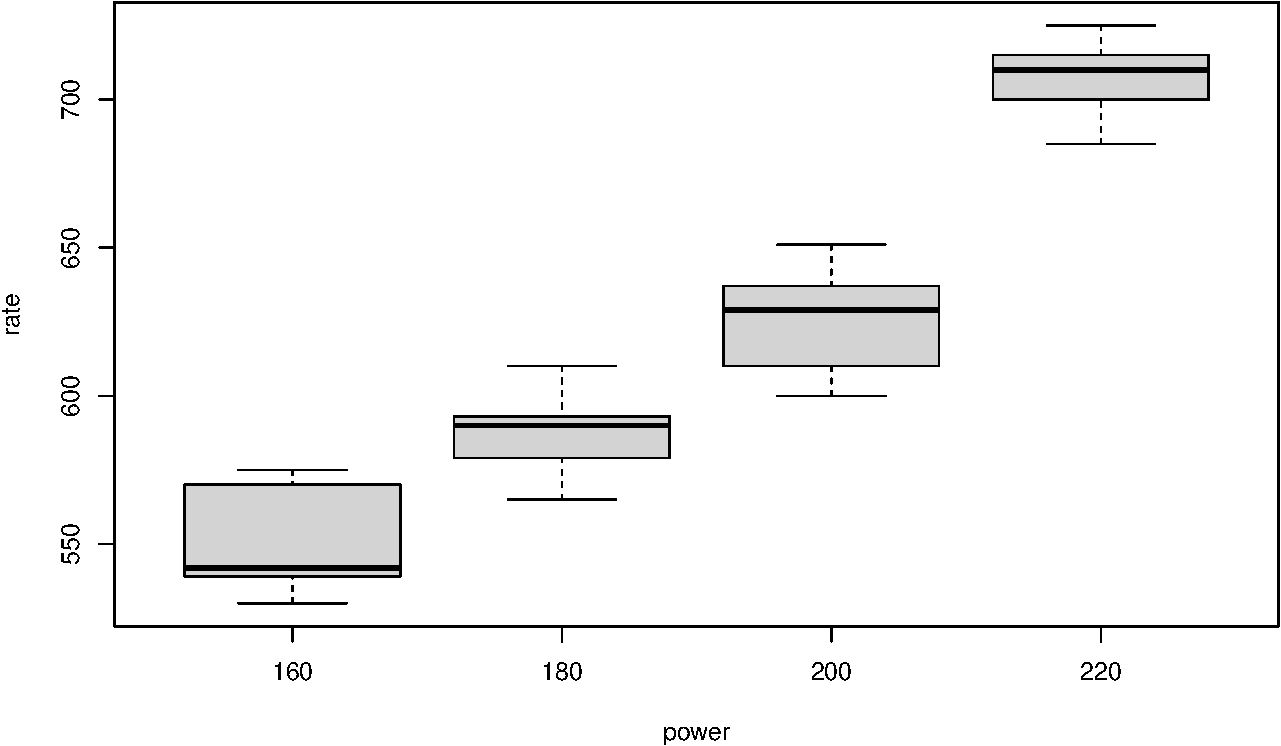
\includegraphics[keepaspectratio]{residuals2_files/figure-latex/unnamed-chunk-1-1.pdf}}

\subsection{Description of Calculated
Columns}\label{description-of-calculated-columns}

The final table compiles several important quantities calculated during
the simulation. Here's what each column represents:

\begin{itemize}
\tightlist
\item
  \(x_i\): The predictor variable, which is simply the index of the
  observation from 1 to 20.
\item
  \(h_i\): The \textbf{leverage} of the i-th observation. It measures
  how influential a point's x-value is in determining the model's fit. A
  higher value indicates a more influential point.
\item
  \(e_i\): The \textbf{ordinary residual}, calculated as the difference
  between the actual value (\(y_i\)) and the predicted value
  (\(\hat{y}_i\)) from the model fit on all data.
\item
  \(\hat{\sigma}\): The \textbf{residual standard error} (or Root Mean
  Square Error) of the full model, representing the typical size of an
  ordinary residual.
\item
  \(e_{i,-i}\): The \textbf{deleted (or LOOCV) residual}. This is the
  difference between the actual value (\(y_i\)) and the value predicted
  for it by a model that was fit on all other data \emph{except} point
  \emph{i}.
\item
  \(\hat{e}*{i,-i}\): This column shows the deleted residual calculated
  using the efficient algebraic shortcut (\(e_i / (1-h*{ii})\)),
  verifying it's identical to the brute-force \(e_{i,-i}\).
\item
  \(\hat{\sigma}_{-i}\): The \textbf{LOOCV residual standard error},
  calculated from a model that was fit after removing observation
  \emph{i}.
\item
  \(\tilde{\sigma}*{-i}\): The \textbf{LOOCV residual standard error},
  calculated from the shortcut formula @eq-sigma*-i.
\item
  \textbf{NS-Full}: The \textbf{Non-studentized Full-Data Residual},
  calculated as the ordinary residual divided by the full model's
  standard error (\(e_i / \hat{\sigma}\)).
\item
  \textbf{NS-LOO}: The \textbf{Non-studentized LOOCV Residual},
  calculated as the deleted residual divided by the corresponding LOOCV
  standard error (\(e_{i,-i} / \hat{\sigma}_{-i}\)).
\item
  \textbf{ST-LOO}: The \textbf{Studentized LOOCV Residual}, calculated
  using the conceptual formula by dividing the deleted residual by its
  true standard error.
\item
  \textbf{ST-Full}: The \textbf{Studentized Full-Data Residual},
  calculated using the efficient shortcut formula, which is provided by
  R's \texttt{rstudent()} function.
\end{itemize}

\begin{Shaded}
\begin{Highlighting}[]
\FunctionTok{library}\NormalTok{(kableExtra)}

\NormalTok{full\_model }\OtherTok{\textless{}{-}} \FunctionTok{lm}\NormalTok{(y }\SpecialCharTok{\textasciitilde{}}\NormalTok{ x, }\AttributeTok{data =}\NormalTok{ full\_data)}
\NormalTok{p }\OtherTok{\textless{}{-}} \FunctionTok{length}\NormalTok{(}\FunctionTok{coef}\NormalTok{(full\_model))}
\NormalTok{leverage   }\OtherTok{\textless{}{-}} \FunctionTok{hatvalues}\NormalTok{(full\_model)}
\NormalTok{e\_full     }\OtherTok{\textless{}{-}} \FunctionTok{resid}\NormalTok{(full\_model)}
\NormalTok{sigma\_hat\_val  }\OtherTok{\textless{}{-}} \FunctionTok{summary}\NormalTok{(full\_model)}\SpecialCharTok{$}\NormalTok{sigma}

\NormalTok{rss\_full }\OtherTok{\textless{}{-}} \FunctionTok{sum}\NormalTok{(e\_full}\SpecialCharTok{\^{}}\DecValTok{2}\NormalTok{)}
\NormalTok{df\_loo }\OtherTok{\textless{}{-}}\NormalTok{ n }\SpecialCharTok{{-}}\NormalTok{ p }\SpecialCharTok{{-}} \DecValTok{1}
\NormalTok{sigma\_minus\_i\_shortcut }\OtherTok{\textless{}{-}} \FunctionTok{sqrt}\NormalTok{((rss\_full }\SpecialCharTok{{-}}\NormalTok{ (e\_full}\SpecialCharTok{\^{}}\DecValTok{2} \SpecialCharTok{/}\NormalTok{ (}\DecValTok{1} \SpecialCharTok{{-}}\NormalTok{ leverage))) }\SpecialCharTok{/}\NormalTok{ df\_loo)}

\CommentTok{\# {-}{-}{-}{-}{-}{-}{-}{-}{-}{-}{-}{-}{-}{-}{-}{-}{-}{-}{-}{-}{-}{-}{-}{-}{-}{-}{-}{-}{-}{-}{-}}
\CommentTok{\# 2) LOOCV quantities (refit n times)}
\CommentTok{\# {-}{-}{-}{-}{-}{-}{-}{-}{-}{-}{-}{-}{-}{-}{-}{-}{-}{-}{-}{-}{-}{-}{-}{-}{-}{-}{-}{-}{-}{-}{-}}
\NormalTok{e\_del\_val }\OtherTok{\textless{}{-}} \FunctionTok{numeric}\NormalTok{(n)}
\NormalTok{sigma\_minus\_i\_val }\OtherTok{\textless{}{-}} \FunctionTok{numeric}\NormalTok{(n)}

\ControlFlowTok{for}\NormalTok{ (i }\ControlFlowTok{in} \DecValTok{1}\SpecialCharTok{:}\NormalTok{n) \{}
\NormalTok{  loocv\_model }\OtherTok{\textless{}{-}} \FunctionTok{lm}\NormalTok{(y }\SpecialCharTok{\textasciitilde{}}\NormalTok{ x, }\AttributeTok{data =}\NormalTok{ full\_data[}\SpecialCharTok{{-}}\NormalTok{i, ])}
\NormalTok{  yhat\_minus  }\OtherTok{\textless{}{-}} \FunctionTok{predict}\NormalTok{(loocv\_model, }\AttributeTok{newdata =}\NormalTok{ full\_data[i, , }\AttributeTok{drop =} \ConstantTok{FALSE}\NormalTok{])}
\NormalTok{  e\_del\_val[i]    }\OtherTok{\textless{}{-}}\NormalTok{ full\_data}\SpecialCharTok{$}\NormalTok{y[i] }\SpecialCharTok{{-}}\NormalTok{ yhat\_minus}
\NormalTok{  sigma\_minus\_i\_val[i] }\OtherTok{\textless{}{-}} \FunctionTok{summary}\NormalTok{(loocv\_model)}\SpecialCharTok{$}\NormalTok{sigma}
\NormalTok{\}}

\CommentTok{\# {-}{-}{-}{-}{-}{-}{-}{-}{-}{-}{-}{-}{-}{-}{-}{-}{-}{-}{-}{-}{-}{-}{-}{-}{-}{-}{-}{-}{-}{-}{-}}
\CommentTok{\# 3) Assemble and round results}
\CommentTok{\# {-}{-}{-}{-}{-}{-}{-}{-}{-}{-}{-}{-}{-}{-}{-}{-}{-}{-}{-}{-}{-}{-}{-}{-}{-}{-}{-}{-}{-}{-}{-}}
\NormalTok{residuals\_df }\OtherTok{\textless{}{-}} \FunctionTok{data.frame}\NormalTok{(}
  \AttributeTok{x =}\NormalTok{ full\_data}\SpecialCharTok{$}\NormalTok{x,}
  \AttributeTok{h =} \FunctionTok{as.numeric}\NormalTok{(leverage),}
  \AttributeTok{e\_i =} \FunctionTok{as.numeric}\NormalTok{(e\_full),}
  \AttributeTok{sigma\_hat =} \FunctionTok{as.numeric}\NormalTok{(sigma\_hat\_val),}
  \AttributeTok{e\_i\_minus\_i =} \FunctionTok{as.numeric}\NormalTok{(e\_del\_val),}
  \AttributeTok{e\_i\_minus\_i\_2 =}\NormalTok{ e\_full}\SpecialCharTok{/}\NormalTok{(}\DecValTok{1} \SpecialCharTok{{-}}\NormalTok{ leverage),}
  \AttributeTok{sigma\_minus\_i =} \FunctionTok{as.numeric}\NormalTok{(sigma\_minus\_i\_val),}
  \AttributeTok{sigma\_minus\_i\_shortcut =} \FunctionTok{as.numeric}\NormalTok{(sigma\_minus\_i\_shortcut),}
  \StringTok{\textasciigrave{}}\AttributeTok{NS{-}Full}\StringTok{\textasciigrave{}} \OtherTok{=}\NormalTok{ e\_full }\SpecialCharTok{/}\NormalTok{ sigma\_hat\_val,}
  \StringTok{\textasciigrave{}}\AttributeTok{NS{-}LOO}\StringTok{\textasciigrave{}} \OtherTok{=}\NormalTok{ e\_del\_val }\SpecialCharTok{/}\NormalTok{ sigma\_minus\_i\_val,}
  \StringTok{\textasciigrave{}}\AttributeTok{ST{-}LOO}\StringTok{\textasciigrave{}} \OtherTok{=}\NormalTok{ e\_del\_val }\SpecialCharTok{/}\NormalTok{ (sigma\_minus\_i\_val }\SpecialCharTok{/} \FunctionTok{sqrt}\NormalTok{(}\DecValTok{1} \SpecialCharTok{{-}}\NormalTok{ leverage)),}
  \StringTok{\textasciigrave{}}\AttributeTok{ST{-}Full}\StringTok{\textasciigrave{}} \OtherTok{=} \FunctionTok{rstudent}\NormalTok{(full\_model)}
\NormalTok{) }\SpecialCharTok{|\textgreater{}}
\NormalTok{  dplyr}\SpecialCharTok{::}\FunctionTok{mutate}\NormalTok{(dplyr}\SpecialCharTok{::}\FunctionTok{across}\NormalTok{(}\FunctionTok{where}\NormalTok{(is.numeric), }\SpecialCharTok{\textasciitilde{}} \FunctionTok{round}\NormalTok{(.x, }\DecValTok{3}\NormalTok{)))}

\CommentTok{\# 4) Create simple display names}
\NormalTok{display\_names }\OtherTok{\textless{}{-}} \FunctionTok{c}\NormalTok{(}\StringTok{"$x\_i$"}\NormalTok{, }\StringTok{"$h\_i$"}\NormalTok{, }\StringTok{"$e\_i$"}\NormalTok{, }\StringTok{"$}\SpecialCharTok{\textbackslash{}\textbackslash{}}\StringTok{hat\{}\SpecialCharTok{\textbackslash{}\textbackslash{}}\StringTok{sigma\}$"}\NormalTok{, }
                   \StringTok{"$e\_\{i,{-}i\}$"}\NormalTok{, }\StringTok{"$}\SpecialCharTok{\textbackslash{}\textbackslash{}}\StringTok{hat\{e\}\_\{i,{-}i\}$"}\NormalTok{,}
                   \StringTok{"$}\SpecialCharTok{\textbackslash{}\textbackslash{}}\StringTok{hat\{}\SpecialCharTok{\textbackslash{}\textbackslash{}}\StringTok{sigma\}\_\{{-}i\}$"}\NormalTok{, }\StringTok{"$}\SpecialCharTok{\textbackslash{}\textbackslash{}}\StringTok{tilde\{}\SpecialCharTok{\textbackslash{}\textbackslash{}}\StringTok{sigma\}\_\{{-}i\}$"}\NormalTok{, }
                   \StringTok{"NS{-}Full"}\NormalTok{, }\StringTok{"NS{-}LOO"}\NormalTok{, }\StringTok{"ST{-}LOO"}\NormalTok{, }\StringTok{"ST{-}Full"}\NormalTok{)}

\CommentTok{\# 5) Display the table}
\ControlFlowTok{if}\NormalTok{ (knitr}\SpecialCharTok{::}\FunctionTok{is\_html\_output}\NormalTok{()) \{}
\NormalTok{  knitr}\SpecialCharTok{::}\FunctionTok{kable}\NormalTok{(}
\NormalTok{    residuals\_df,}
    \AttributeTok{caption =} \StringTok{"Residual variants"}\NormalTok{,}
    \AttributeTok{col.names =}\NormalTok{ display\_names,}
    \AttributeTok{align =} \StringTok{"r"}\NormalTok{,}
    \AttributeTok{escape =} \ConstantTok{FALSE}
\NormalTok{  )}
\NormalTok{\} }\ControlFlowTok{else}\NormalTok{ \{}
\NormalTok{  knitr}\SpecialCharTok{::}\FunctionTok{kable}\NormalTok{(}
\NormalTok{    residuals\_df,}
    \AttributeTok{caption =} \StringTok{"Residual variants."}\NormalTok{,}
    \AttributeTok{col.names =}\NormalTok{ display\_names,}
    \AttributeTok{align =} \StringTok{"r"}\NormalTok{,}
    \AttributeTok{format =} \StringTok{"latex"}\NormalTok{,}
    \AttributeTok{booktabs =} \ConstantTok{TRUE}\NormalTok{,}
    \AttributeTok{escape =} \ConstantTok{FALSE}
\NormalTok{  ) }\SpecialCharTok{|\textgreater{}}
    \FunctionTok{kable\_styling}\NormalTok{(}\AttributeTok{latex\_options =} \StringTok{"scale\_down"}\NormalTok{)}
\NormalTok{\}}
\end{Highlighting}
\end{Shaded}

\begin{table}
\centering
\caption{\label{tab:plaintext}Residual variants.}
\centering
\resizebox{\ifdim\width>\linewidth\linewidth\else\width\fi}{!}{
\begin{tabular}[t]{rrrrrrrrrrrr}
\toprule
$x_i$ & $h_i$ & $e_i$ & $\hat{\sigma}$ & $e_{i,-i}$ & $\hat{e}_{i,-i}$ & $\hat{\sigma}_{-i}$ & $\tilde{\sigma}_{-i}$ & NS-Full & NS-LOO & ST-LOO & ST-Full\\
\midrule
1 & 0.186 & 20.156 & 7.155 & 24.753 & 24.753 & 4.986 & 4.986 & 2.817 & 4.964 & 4.479 & 4.479\\
2 & 0.159 & -7.684 & 7.155 & -9.133 & -9.133 & 7.077 & 7.077 & -1.074 & -1.290 & -1.184 & -1.184\\
3 & 0.135 & 1.769 & 7.155 & 2.045 & 2.045 & 7.348 & 7.348 & 0.247 & 0.278 & 0.259 & 0.259\\
4 & 0.114 & -5.163 & 7.155 & -5.824 & -5.824 & 7.242 & 7.242 & -0.722 & -0.804 & -0.757 & -0.757\\
5 & 0.095 & -4.360 & 7.155 & -4.820 & -4.820 & 7.278 & 7.278 & -0.609 & -0.662 & -0.630 & -0.630\\
\addlinespace
6 & 0.080 & 4.078 & 7.155 & 4.434 & 4.434 & 7.290 & 7.290 & 0.570 & 0.608 & 0.583 & 0.583\\
7 & 0.068 & -1.684 & 7.155 & -1.808 & -1.808 & 7.351 & 7.351 & -0.235 & -0.246 & -0.237 & -0.237\\
8 & 0.059 & -9.805 & 7.155 & -10.425 & -10.425 & 6.943 & 6.943 & -1.370 & -1.502 & -1.456 & -1.456\\
9 & 0.053 & -6.406 & 7.155 & -6.767 & -6.767 & 7.188 & 7.188 & -0.895 & -0.941 & -0.916 & -0.916\\
10 & 0.050 & -4.691 & 7.155 & -4.940 & -4.940 & 7.270 & 7.270 & -0.656 & -0.679 & -0.662 & -0.662\\
\addlinespace
11 & 0.050 & 4.167 & 7.155 & 4.388 & 4.388 & 7.289 & 7.289 & 0.582 & 0.602 & 0.587 & 0.587\\
12 & 0.053 & 0.354 & 7.155 & 0.374 & 0.374 & 7.362 & 7.362 & 0.049 & 0.051 & 0.049 & 0.049\\
13 & 0.059 & 1.068 & 7.155 & 1.135 & 1.135 & 7.358 & 7.358 & 0.149 & 0.154 & 0.150 & 0.150\\
14 & 0.068 & 0.126 & 7.155 & 0.135 & 0.135 & 7.363 & 7.363 & 0.018 & 0.018 & 0.018 & 0.018\\
15 & 0.080 & -2.698 & 7.155 & -2.934 & -2.934 & 7.331 & 7.331 & -0.377 & -0.400 & -0.384 & -0.384\\
\addlinespace
16 & 0.095 & 9.525 & 7.155 & 10.530 & 10.530 & 6.951 & 6.951 & 1.331 & 1.515 & 1.441 & 1.441\\
17 & 0.114 & 3.588 & 7.155 & 4.048 & 4.048 & 7.305 & 7.305 & 0.501 & 0.554 & 0.522 & 0.522\\
18 & 0.135 & -8.225 & 7.155 & -9.504 & -9.504 & 7.044 & 7.044 & -1.150 & -1.349 & -1.255 & -1.255\\
19 & 0.159 & 5.623 & 7.155 & 6.684 & 6.684 & 7.211 & 7.211 & 0.786 & 0.927 & 0.850 & 0.850\\
20 & 0.186 & 0.261 & 7.155 & 0.321 & 0.321 & 7.363 & 7.363 & 0.037 & 0.044 & 0.039 & 0.039\\
\bottomrule
\end{tabular}}
\end{table}

\begin{Shaded}
\begin{Highlighting}[]
\FunctionTok{library}\NormalTok{(dplyr)}
\FunctionTok{library}\NormalTok{(tidyr)}
\FunctionTok{library}\NormalTok{(ggplot2)}
\FunctionTok{library}\NormalTok{(knitr)}

\CommentTok{\# Prepare data for plotting}
\NormalTok{plot\_df }\OtherTok{\textless{}{-}}\NormalTok{ residuals\_df }\SpecialCharTok{|\textgreater{}}
\NormalTok{  dplyr}\SpecialCharTok{::}\FunctionTok{select}\NormalTok{(}
\NormalTok{    x,}
\NormalTok{    NS.Full,}
\NormalTok{    NS.LOO,}
\NormalTok{    ST.LOO,}
\NormalTok{    ST.Full}
\NormalTok{  ) }\SpecialCharTok{|\textgreater{}}
\NormalTok{  tidyr}\SpecialCharTok{::}\FunctionTok{pivot\_longer}\NormalTok{(}
    \AttributeTok{cols =} \SpecialCharTok{{-}}\NormalTok{x,}
    \AttributeTok{names\_to =} \StringTok{"residual\_type"}\NormalTok{,}
    \AttributeTok{values\_to =} \StringTok{"residual\_value"}
\NormalTok{  )}

\NormalTok{shape\_map }\OtherTok{\textless{}{-}} \FunctionTok{c}\NormalTok{(}
  \AttributeTok{NS.Full =} \DecValTok{16}\NormalTok{,}
  \AttributeTok{NS.LOO  =} \DecValTok{1}\NormalTok{,}
  \AttributeTok{ST.LOO  =} \DecValTok{6}\NormalTok{,}
  \AttributeTok{ST.Full =} \DecValTok{10}
\NormalTok{)}

\NormalTok{labels\_map }\OtherTok{\textless{}{-}} \FunctionTok{c}\NormalTok{(}
  \AttributeTok{NS.Full =} \StringTok{"NS{-}Full"}\NormalTok{,}
  \AttributeTok{NS.LOO  =} \StringTok{"NS{-}LOO"}\NormalTok{,}
  \AttributeTok{ST.LOO  =} \StringTok{"ST{-}LOO"}\NormalTok{,}
  \AttributeTok{ST.Full =} \StringTok{"ST{-}Full"}
\NormalTok{)}

\NormalTok{color\_map }\OtherTok{\textless{}{-}} \FunctionTok{c}\NormalTok{(}
  \AttributeTok{NS.Full =} \StringTok{"\#1f77b4"}\NormalTok{,}
  \AttributeTok{NS.LOO  =} \StringTok{"\#ff7f0e"}\NormalTok{,}
  \AttributeTok{ST.LOO  =} \StringTok{"\#2ca02c"}\NormalTok{,}
  \AttributeTok{ST.Full =} \StringTok{"\#d62728"}
\NormalTok{)}

\FunctionTok{ggplot}\NormalTok{(}
\NormalTok{  plot\_df,}
  \FunctionTok{aes}\NormalTok{(}\AttributeTok{x =}\NormalTok{ x, }\AttributeTok{y =}\NormalTok{ residual\_value,}
      \AttributeTok{shape =}\NormalTok{ residual\_type, }\AttributeTok{color =}\NormalTok{ residual\_type, }\AttributeTok{group =}\NormalTok{ residual\_type)}
\NormalTok{) }\SpecialCharTok{+}
  \FunctionTok{geom\_hline}\NormalTok{(}\AttributeTok{yintercept =} \DecValTok{0}\NormalTok{, }\AttributeTok{linetype =} \StringTok{"dashed"}\NormalTok{) }\SpecialCharTok{+}
  \FunctionTok{geom\_point}\NormalTok{(}\AttributeTok{size =} \DecValTok{3}\NormalTok{, }\AttributeTok{stroke =} \FloatTok{1.2}\NormalTok{) }\SpecialCharTok{+}
  \FunctionTok{scale\_shape\_manual}\NormalTok{(}
    \AttributeTok{values =}\NormalTok{ shape\_map,}
    \AttributeTok{breaks =} \FunctionTok{names}\NormalTok{(labels\_map),}
    \AttributeTok{labels =} \FunctionTok{unname}\NormalTok{(labels\_map),}
    \AttributeTok{name =} \StringTok{"Residual Type"}
\NormalTok{  ) }\SpecialCharTok{+}
  \FunctionTok{scale\_color\_manual}\NormalTok{(}
    \AttributeTok{values =}\NormalTok{ color\_map,}
    \AttributeTok{breaks =} \FunctionTok{names}\NormalTok{(labels\_map),}
    \AttributeTok{labels =} \FunctionTok{unname}\NormalTok{(labels\_map),}
    \AttributeTok{name =} \StringTok{"Residual Type"}
\NormalTok{  ) }\SpecialCharTok{+}
  \FunctionTok{labs}\NormalTok{(}
    \AttributeTok{title =} \StringTok{"Four Residual Variants vs x"}\NormalTok{,}
    \AttributeTok{x =} \StringTok{"x\_i"}\NormalTok{,}
    \AttributeTok{y =} \StringTok{"Residual value"}
\NormalTok{  ) }\SpecialCharTok{+}
  \FunctionTok{theme\_bw}\NormalTok{() }\SpecialCharTok{+}
  \FunctionTok{theme}\NormalTok{(}
    \AttributeTok{legend.position =} \StringTok{"right"}\NormalTok{,}
    \AttributeTok{legend.title =} \FunctionTok{element\_text}\NormalTok{(}\AttributeTok{face =} \StringTok{"bold"}\NormalTok{)}
\NormalTok{  )}
\end{Highlighting}
\end{Shaded}

\begin{figure}
\centering
\pandocbounded{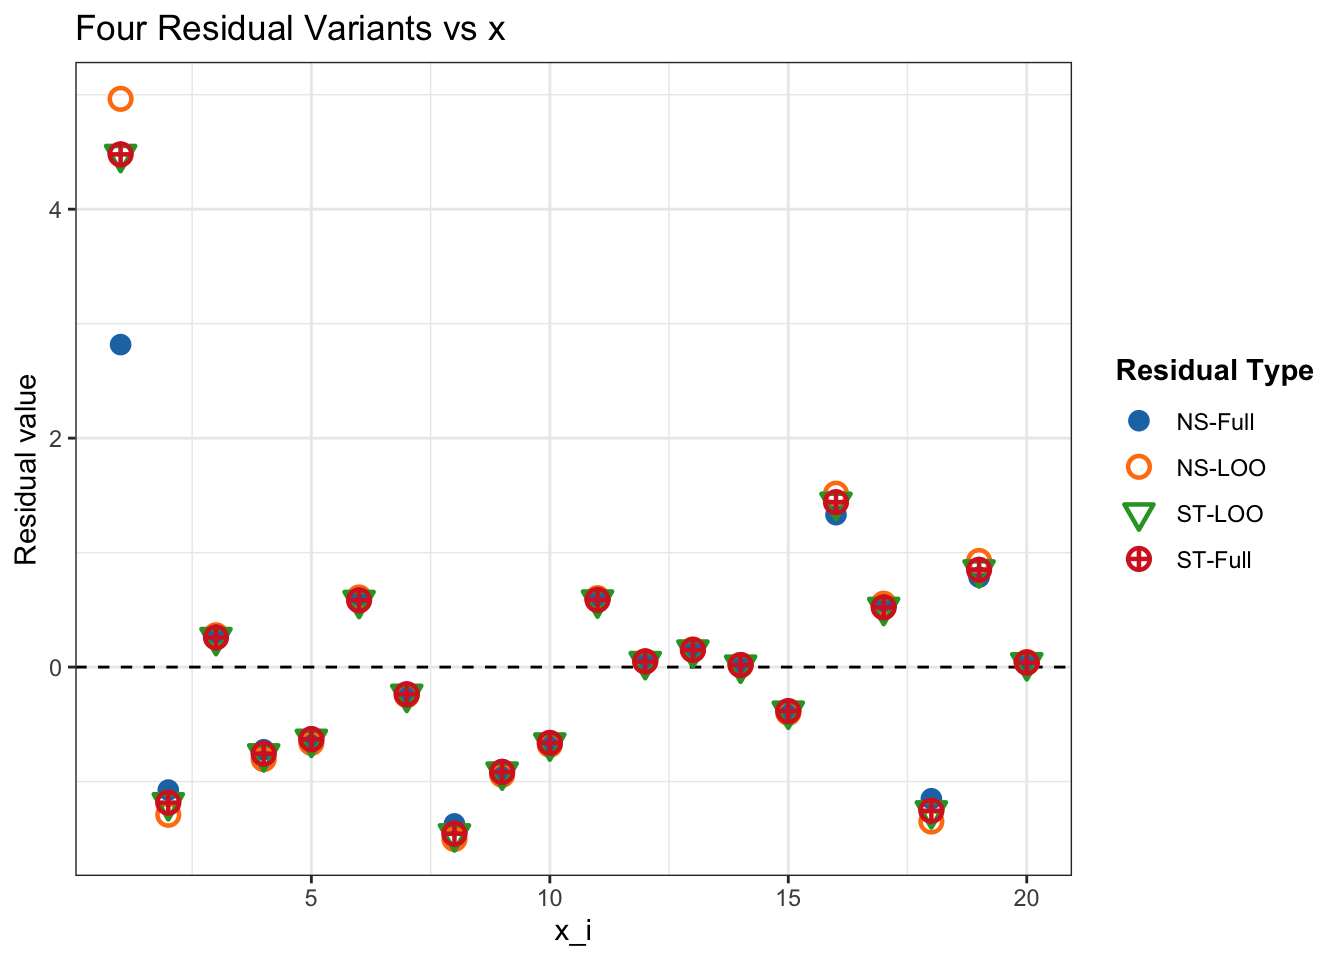
\includegraphics[keepaspectratio,alt={Four residual variants plotted against the predictor variable x.}]{residuals2_files/figure-latex/plot-four-residuals-new-names-1.pdf}}
\caption{Four residual variants plotted against the predictor variable
x.}
\end{figure}

From the above simulation results, we observe the following important
facts:

\begin{itemize}
\item
  \textbf{Leverage and Influence:} The simulation confirms that leverage
  (\(h_{ii}\)) measures an observation's influence on the model's
  coefficients. It shows that points with higher leverage pull the
  regression line toward them, resulting in smaller, deceptively
  conservative full-data residuals (\(e_i\)).
\item
  \textbf{Conservative Residuals:} The study highlights that the
  ordinary residual (\(e_i\)) is a ``conservative'' measure of error
  because its value for an outlier is systematically reduced by that
  same outlier's influence on the model.
\item
  \textbf{Identity Verification:} The numerical results validated the
  key algebraic identity that connects the full-data residual (\(e_i\))
  to the leave-one-out (deleted) residual (\(e_{i,-i}\)), as well as the
  identity for calculating the LOOCV standard error
  (\(\hat{\sigma}_{-i}\)) from the full model's statistics. This
  demonstrates that all key LOOCV errors can be calculated efficiently
  from a single model fit.
\item
  \textbf{Effective Studentization:} The final step of studentization,
  which uses leverage to properly scale the residuals, is shown to be
  crucial. It successfully transforms the residuals into a reliable
  diagnostic tool with a constant variance across all predictor values
  (\(x_i\)), causing them to behave much more like a standard normal or
  t-distribution.
\end{itemize}

\section*{Appendix:}\label{appendix}
\addcontentsline{toc}{section}{Appendix:}

\section{Key Identities for Efficient Calculation of LOOCV Residuals and
Noise
Variance}\label{key-identities-for-efficient-calculation-of-loocv-residuals-and-noise-variance}

The power of modern regression diagnostics comes from algebraic
shortcuts that allow us to find the results of a leave-one-out process
without the computational cost of refitting the model \emph{n} times.
The following two identities are fundamental to this efficiency.

\subsection{\texorpdfstring{Finding the LOOCV Residual (\(e_{i,-i}\))
from the Ordinary Residual
(\(e_i\))}{Finding the LOOCV Residual (e\_\{i,-i\}) from the Ordinary Residual (e\_i)}}\label{finding-the-loocv-residual-e_i-i-from-the-ordinary-residual-e_i}

This identity shows that we can find the ``pure'' leave-one-out residual
using only the results from the single model fit on all data.

\[e_{i,-i} = \frac{e_i}{1 - h_{ii}}\] \{\#eq-key\}

\subsection{\texorpdfstring{Finding the LOOCV Standard Error
(\(\hat{\sigma}_{-i}\)) from the Full-Model Standard Error
(\(\hat{\sigma}\))}{Finding the LOOCV Standard Error (\textbackslash hat\{\textbackslash sigma\}\_\{-i\}) from the Full-Model Standard Error (\textbackslash hat\{\textbackslash sigma\})}}\label{finding-the-loocv-standard-error-hatsigma_-i-from-the-full-model-standard-error-hatsigma}

Similarly, this formula provides an efficient shortcut to see how the
model's overall error changes when a single point is removed.

\[\hat{\sigma}*{-i} = \sqrt{\frac{(n-p)\hat{\sigma}^2 - \frac{e_i^2}{1-h*{ii}}}{n-p-1}}\]
\{\#eq-sigma\_-i\}

The derivation of this formula relies on first proving the relationship
between the full model's Residual Sum of Squares (\(RSS\)) and the
leave-one-out version (\(RSS_{-i}\)).

\begin{enumerate}
\def\labelenumi{\arabic{enumi}.}
\item
  \textbf{Start with the definition} of the leave-one-out residual sum
  of squares: \[
  RSS_{-i} = \sum_{k \neq i} (y_k - \mathbf{x}*k^T\hat{\beta}*{-i})^2
  \]
\item
  \textbf{Introduce the key identity} that relates the leave-one-out
  coefficient vector (\(\hat{\beta}*{-i}\)) to the full model's
  coefficient vector (\(\hat{\beta}\)): \[
  \hat{\beta}*{-i} = \hat{\beta} - (X^TX)^{-1}\mathbf{x}*i \frac{e_i}{1 - h*{ii}}
  \]
\item
  \textbf{Substitute this identity} into the expression for a generic
  leave-one-out residual,
  \(e_{k,-i} = y_k - \mathbf{x}*k^T\hat{\beta}*{-i}\). After
  simplification, this yields: \[
  e_{k,-i} = e_k + h_{ki} \frac{e_i}{1 - h_{ii}}
  \] where \(e_k\) is the ordinary residual and \(h_{ki}\) is the
  \((k,i)\)-th element of the hat matrix.
\item
  \textbf{Substitute this back into the definition of} \(RSS_{-i}\).
  After expanding the squared term and performing the summation (which
  involves considerable but standard matrix algebra), the expression
  simplifies to the elegant result: \[
  RSS_{-i} = RSS - \frac{e_i^2}{1 - h_{ii}}
  \]
\item
  \textbf{Finally, derive the formula for} \(\hat{\sigma}*{-i}\). We
  know that \(\hat{\sigma}^2*{-i} = \frac{RSS_{-i}}{n-p-1}\) and that
  \(RSS = (n-p)\hat{\sigma}^2\). By substituting the result from Step 4,
  we arrive at the formula for the variance, and taking the square root
  gives us the standard error. ✅
\end{enumerate}

\end{document}
